This section will explain how the model was trained, validated, and tested. Several adjustments were
made to improve the model's prediction accuracy. For the training process, the model was trained with
training data sets and validated with validation data sets. On the other hand, testing data sets are
completely different from the training and validation data sets.
The number of training data sets are 47930 and validation sets are 5325. Also, the number of testing
datasets is 5564. The validation set size is
roughly 10 percent of the training data sets. Five different experiment took place to improve the
prediction accuracy. In order to see the difference in the experiment, the model was trained with two
different learning rate and the number of epochs; Learning rate was 0.0001 and 0.00001; The number of
epochs are 17, 21, and 27. Finally, one batch of data sets contain 32 data sets.
\newline
\newline
\indent
To begin with, during the training process, the goal is to minimize the validation loss. Therefore,
training with different independent variables such as epoch sizes and learning rates produced the various
accuracy when predicting. The training processes and the results of prediction with the prediction accuracy are
provided in the figures below. The size of increase in the number of iterations are limited in this experiemnt
due to the  limitation in computational power.
\newline

    \begin{figure}
        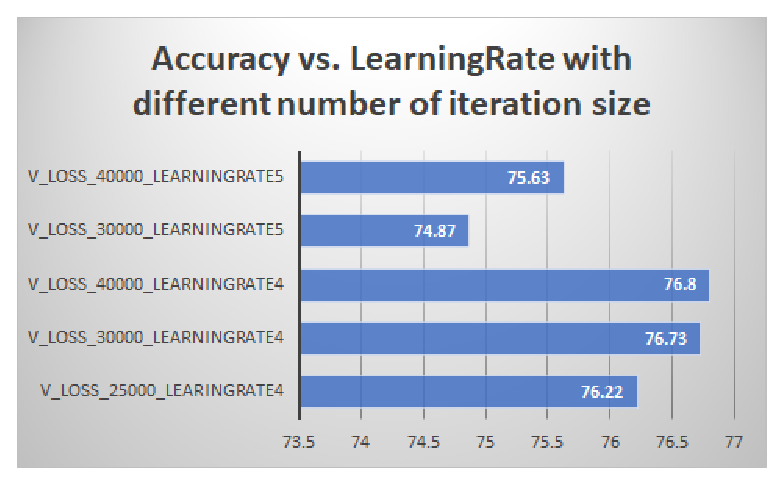
\includegraphics[width=\textwidth, scale=0.25]{val_acc.eps}
        \caption{Accuracy of the model in terms of learning rate and the number of iterations.}
        \label{Figure2}
    \end{figure}


According to model accuracy data in the Figure \ref{Figure2}, the model has the highest accuracy when trained
with learning rate of 0.0001 and 40000 number of iterations. Originally, the model was trained with same learning rate, but
25000 number of iterations. The reason behind is that validation loss was observed to be the minimum. However, although
increasing number of iterations produces less optimized validation losss, it trained the model to have more accurate
prediction rate.
\newline
\newline
\indent
Moreover, trainings with learning rate of 0.00001 produce lower accuracy models compare to models trained with 0.0001.
Due to slower learning rate, the model requires higher number of training iterations to become more accurate. In this
context, this cannot be achievable due to lacking computational power.
\newline
\newline
\indent
Finally, it is observed that the prediction accuracy is distorted. For instance, the input data shows the same image for
lower case 'z' and upper case 'Z'. There are several alphabet characters causing prediction accuracy to be lower than expected.
This type of errors are not in the scope of this project. Therefore, accounting computational power and errorneous input data,
the model's prediction accuracy is high, roughly 76 percent, in that it can classify the 58 character images regardless of font types.


